%!TEX root = ../pres - final.tex

\section{Metodología propuesta}

\begin{frame}{Metodología propuesta}
  \begin{figure}[bth]
    \centerline
    {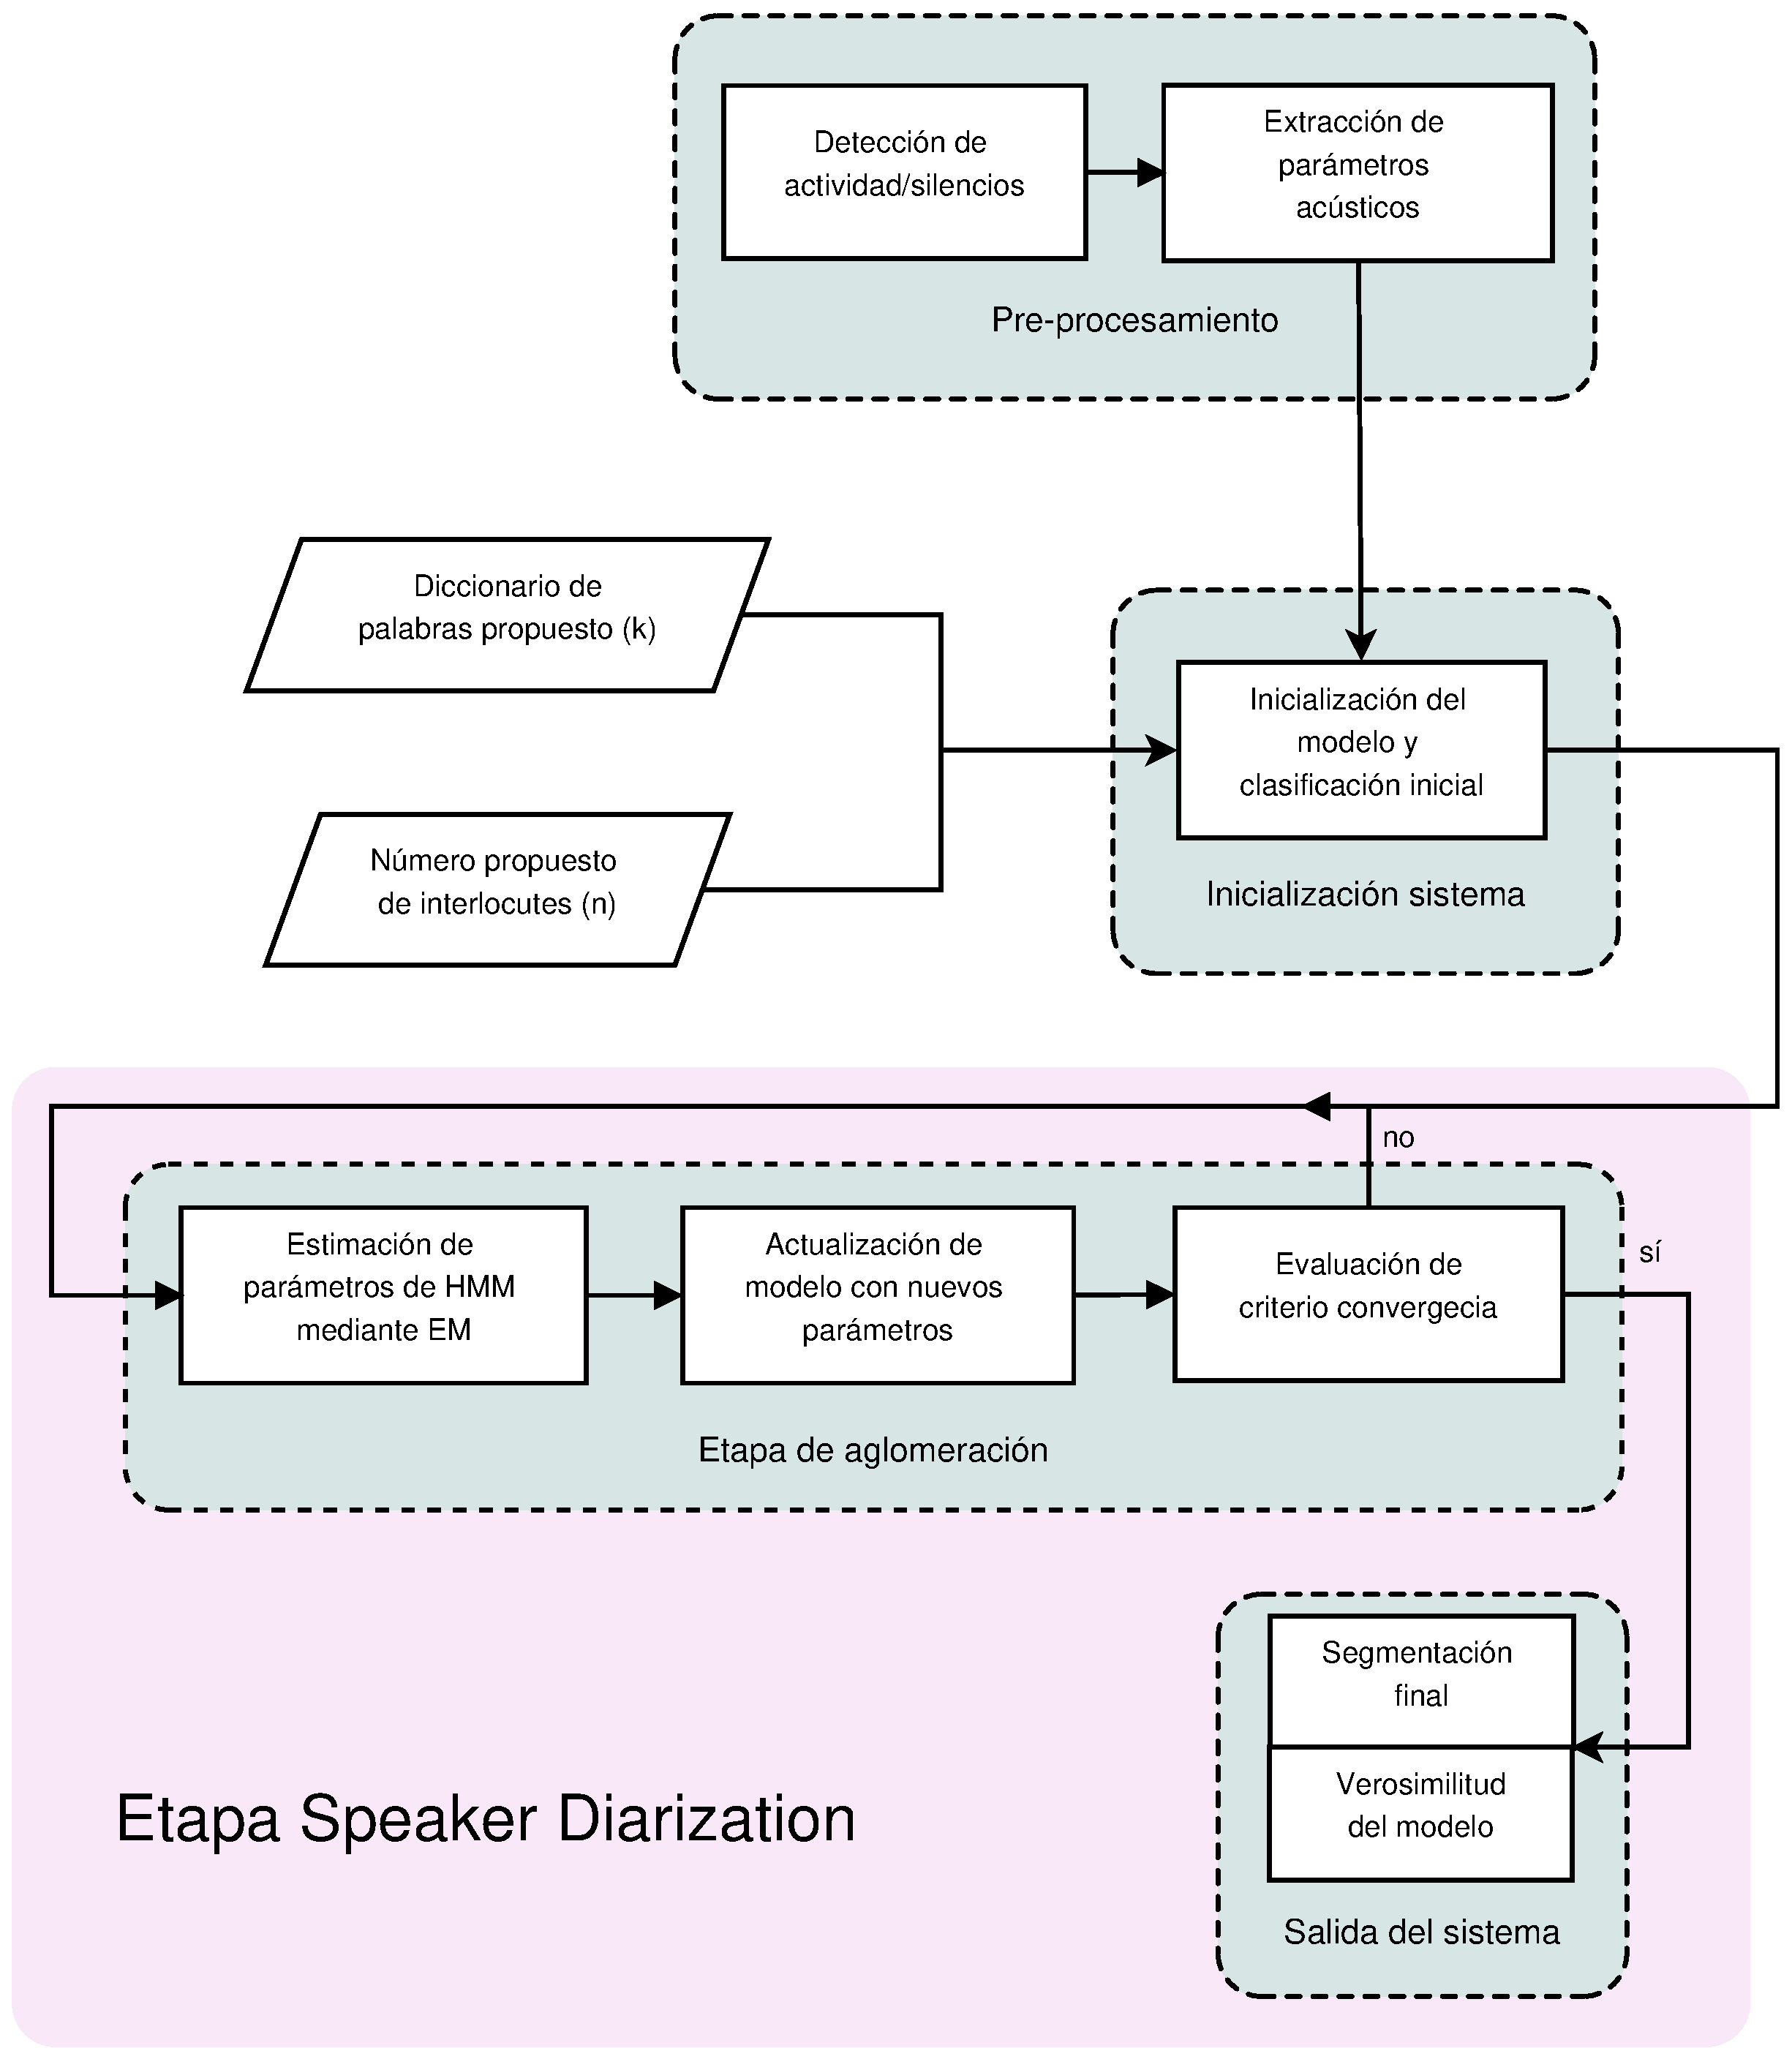
\includegraphics[width=0.6\linewidth]{gfx/general_flow}} \quad
    \caption{Esquema general.}
    \label{fig:esquema}
  \end{figure}
\end{frame}

% \begin{frame}{Selección de modelo realizada}
%   \begin{itemize} 
%     \itemsep1em

%     \item Este proceso se realizara en dos partes: 

%       \begin{itemize} 
%         \itemsep0.8em
%         \item Exploración de todo el espacio de soluciones y reducción de posibles modelos ganadores.
%         \item Selección de mejor modelo entre los candidatos resultantes.
%       \end{itemize}  
%     \end{itemize}   
% \end{frame}

\begin{frame}{Selección de modelo realizada}{Exploración}
  \begin{itemize} 
    \itemsep1em

    \item
    Se estimará BIC de todos los HMM propuestos para generar una curva de selección. 

    \item Como se verá en las pruebas, es necesario introducir un término de regularización en BIC para que la penalización del modelo corresponda con las log-verosimilitudes obtenidas. 
    \begin{equation}
    BIC_{\lambda}(\mc{M}) = 2 \mc{L}_{max}(\mc{M}) - \lambda \cdot log N \cdot dim(M)
    \end{equation}

    \item Se deberá encontrar el valor adecuado para $\lambda$ que penalice de buena forma los modelos. 
    \end{itemize}   
\end{frame}    

\begin{frame}{Selección de modelo realizada}{Exploración}
  \begin{itemize} 
    \itemsep1em
    \item Para escoger el valor adecuado de $\lambda$ se realizará un análisis de sensibilidad, generando múltiples curvas de selección BIC con diferentes valores de $\lambda$. 

    \item Se buscará la región de inflexión que divide a la superficie anterior en dos: en la primera parte de la superficie. 
    %, el valor de $\lambda$ será pequeño, por lo que siempre tendrán una mayor verosimilitud los modelos con más parámetros; mientras que en la segunda parte, la penalización sera muy grande, y se escogerán siempre los modelos más sencillos, sin darle tomar en cuenta su verosimilitud.

    \item Calculando el gradiente de la superficie generada por las funciones BIC, se buscará la región asociada a un $\lambda$ en el que la suma de los valores absolutos sea menor. 

    \item Una vez que se logre seleccionar el $\lambda$ adecuado de regularización, se procede a evaluar su curva BIC asociada y de ahí se obtiene al modelo ganador o un subconjunto de posibles ganadores.
  \end{itemize}   
\end{frame}    

\begin{frame}{Selección de modelo realizada}{Selección}
  \begin{itemize} 
    \itemsep1em

    \item Luego se realizará un proceso de refinamiento en caso de que se tengan varios modelos posibles. 

    \item Se formarán pares de modelos que se deseen comparar, y se estimará su LLR, que se denominará como $LLR_{obs}$. 

    \item Luego, mediante bootstrap paramétrico se hará una prueba de hipótesis para comproar cuál modelo es más adecuado para los datos.

    \item De esta forma, se pueden realizar pruebas de hipótesis para los modelos candidatos, e ir rechazando modelos de acuerdo al análisis propuesto. 

  \end{itemize}   
\end{frame}    

